\documentclass[11pt]{article}

% --- Packages ---
\usepackage[margin=1in]{geometry}
\usepackage{amsmath,amssymb}
\usepackage{graphicx}
\usepackage{hyperref}
\usepackage{booktabs}
\usepackage{xcolor}
\usepackage{microtype}
\usepackage{authblk}
\usepackage[numbers,sort&compress]{natbib}
\usepackage{algorithm}
\usepackage{algpseudocode}
\usepackage{listings}
\usepackage{caption}
\usepackage{subcaption}
\usepackage{tikz}
\usepackage{pgfplots}
\pgfplotsset{compat=1.18}

\definecolor{shblue}{RGB}{30,90,200}
\hypersetup{colorlinks=true, linkcolor=shblue, citecolor=shblue, urlcolor=shblue}

% --- Title & Authors ---
\title{
  \textbf{Genesis Directive: Contrastive Latent Plan Coupling for\\
  Structure-Sensitive Language Generation}
}

\author[1]{Tino Musikavanhu}
\affil[1]{Safehaven Labs}

\date{March 2026 \quad\textit{(Preprint — submitted to arXiv)}}

% ============================================================
\begin{document}
\maketitle

\begin{abstract}
We introduce \textbf{Genesis Directive}, a framework for investigating the representation geometry of explicitly coupled latent planning channels in autoregressive language generation. We couple a \emph{diffusion-based latent planner} to an \emph{autoregressive decoder} through a learned projection bridge. By isolating the optimization of semantic compatibility from order-aware structural sensitivity, we uncover a fundamental architectural tension: mechanisms capable of inducing strong structural separation simultaneously destabilize decoder-compatible semantic geometry. Our experiments on WikiText-2 define three distinct representational regimes: (1) \emph{Pure Alignment}, which establishes strong semantic utility ($\Delta_z = +1.61$ nats); (2) \emph{Full Contrastive Optimization}, which induces strong structural sensitivity ($S = +1.37$ nats) but collapses the semantic manifold; and (3) \emph{Orthogonal Dual-Head architectures}, which preserve semantic stability but lack the representational capacity for deep structural separation. We conclude that semantic compatibility and structural discrimination occupy competing optimization regimes in latent-prefix coupling, necessitating deeper architectural unbinding than shallow gating or additive orthogonalization can provide. Code and checkpoints are available at \url{https://github.com/safehavenlabs/genesis-directive}.
\end{abstract}

% ============================================================
\section{Introduction}
\label{sec:intro}

Large language models (LLMs) generate text autoregressively, conditioning each
token on the preceding context.
While powerful, this paradigm offers no principled mechanism for high-level
planning prior to generation.
Humans, by contrast, tend to form an abstract outline before writing — a
semantic skeleton that guides word-by-word realisation.

Diffusion language models such as LLaDA~\citep{nie2025llada} operate in
\emph{latent space}, iteratively denoising a full-sequence representation.
We ask: are explicit latent planning channels a required inductive bias for 
coherence under autoregressive constraints? Can an externalized latent structure 
encode global ordering constraints that an autoregressive decoder actively binds to?

This motivates the \textbf{Genesis Directive} framework
(Figure~\ref{fig:architecture}).
Our contributions are:

\begin{enumerate}
  \item A framework for mapping the representation geometry of structural dependency, pairing a frozen diffusion planner with a LoRA-adapted autoregressive decoder via a learned \emph{projection bridge}.
  \item The \textbf{Wrong-Structure Penalty} ($S$), an evaluation metric that isolates structural asymmetry, providing a stable measure of structural dependency regardless of semantic noise floors.
  \item An \textbf{order-aware self-shuffle contrastive loss} that operationalises global ordering constraints in the latent projection manifold.
  \item Experimental mapping of three distinct optimization regimes that empirically prove semantic compatibility and structural discrimination compete for the same latent coordinates.
  \item A systematic mixed-precision training protocol for Apple MPS that eliminates fp16 NaN gradients entirely without requiring a decoder backward pass.
\end{enumerate}

% ============================================================
\section{Background}
\label{sec:background}

\subsection{Diffusion Language Models}

Diffusion LMs define a forward process that corrupts a sequence $x_0$ with
Gaussian or masking noise over $T$ steps, and learn a reverse process to
recover the original.
LLaDA~\citep{nie2025llada} performs masked diffusion directly over token IDs,
producing hidden representations $Z \in \mathbb{R}^{L \times d_p}$ that encode
full-sequence semantics without the strict left-to-right inductive bias of
autoregressive models.

\subsection{Soft Prompting and Prefix Tuning}

Prefix tuning~\citep{li2021prefix} prepends learnable continuous vectors to
the decoder's embedding sequence, steering generation without fine-tuning base
model weights.
We extend this idea by replacing the learnable prefix with a
\emph{task-conditioned latent plan} produced dynamically by the diffusion planner.

\subsection{Contrastive Representation Learning}

Contrastive methods encourage representations to be similar for semantically
related inputs and dissimilar for unrelated ones.
SimCLR~\citep{chen2020simple} and InfoNCE~\citep{oord2018representation}
have been widely applied in vision; their application to discrete sequence
structure in language models is less explored.
Our self-shuffle contrastive loss is a novel adaptation that specifically
penalises insensitivity to \emph{token order} within the latent plan.

% ============================================================
\section{Method}
\label{sec:method}

\subsection{Architecture Overview}
\label{sec:arch}

\begin{figure}[h]
  \centering
  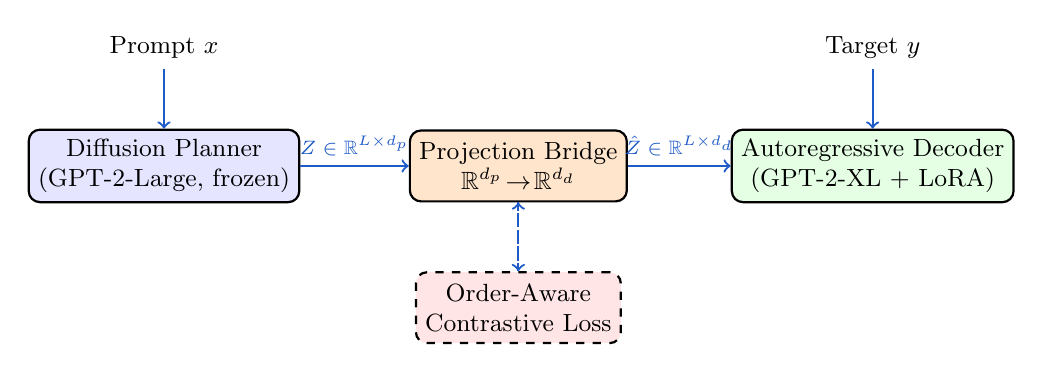
\begin{tikzpicture}[
    box/.style={draw, rounded corners=4pt, minimum width=2.6cm, minimum height=0.9cm,
                thick, font=\small, align=center},
    arr/.style={->, thick, shblue}
  ]
    % Planner
    \node[box, fill=blue!10] (planner) at (0,0) {Diffusion Planner\\(GPT-2-Large, frozen)};
    % Projection
    \node[box, fill=orange!20] (proj) at (4.5,0) {Projection Bridge\\$\mathbb{R}^{d_p} \!\to\! \mathbb{R}^{d_d}$};
    % Decoder
    \node[box, fill=green!10] (decoder) at (9,0) {Autoregressive Decoder\\(GPT-2-XL + LoRA)};
    % Text input
    \node[font=\small] (prompt) at (0, 1.5) {Prompt $x$};
    \node[font=\small] (text) at (9, 1.5) {Target $y$};
    % Loss
    \node[box, fill=red!10, dashed] (loss) at (4.5,-1.8) {Order-Aware\\Contrastive Loss};
    % Arrows
    \draw[arr] (prompt) -- (planner);
    \draw[arr] (planner) -- node[above, font=\scriptsize]{$Z \in \mathbb{R}^{L \times d_p}$} (proj);
    \draw[arr] (proj) -- node[above, font=\scriptsize]{$\hat{Z} \in \mathbb{R}^{L \times d_d}$} (decoder);
    \draw[arr] (text) -- (decoder);
    \draw[arr, dashed] (proj) -- (loss);
    \draw[arr, dashed] (loss) -- (proj);
  \end{tikzpicture}
  \caption{Genesis Directive architecture. The frozen diffusion planner produces a
  latent plan $Z$; the projection bridge maps it to the decoder's embedding space;
  the decoder generates text conditioned on the soft prefix $\hat{Z}$.
  The contrastive loss trains the bridge in fp32 without a decoder backward pass.}
  \label{fig:architecture}
\end{figure}

\paragraph{Planner.}
We use GPT-2-Large~\citep{radford2019language} as a masked-diffusion surrogate
following LLaDA~\citep{nie2025llada}:
we iteratively denoise masked tokens using GPT-2 hidden states as the latent
trajectory, extracting the final hidden-state sequence as the plan $Z$.
Given a prompt $x$, the planner produces
$Z = f_\theta(x) \in \mathbb{R}^{L \times 1280}$, where $L$ is the sequence length.

\paragraph{Projection Bridge.}
A learned MLP maps $Z$ from the planner dimension $d_p = 1280$ to the decoder
dimension $d_d = 1600$:
\begin{equation}
  \hat{Z} = g_\phi\!\left(\mathrm{LayerNorm}(Z)\right), \quad
  g_\phi : \mathbb{R}^{d_p} \to \mathbb{R}^{d_d}.
  \label{eq:proj}
\end{equation}
We evaluate four architectures for $g_\phi$ (Section~\ref{sec:exp4}).

\paragraph{Decoder.}
GPT-2-XL~\citep{radford2019language} with LoRA adapters~\citep{hu2021lora}
($r=8$, target \texttt{c\_attn}) is used as the decoder.
The soft prefix is formed by concatenating $\hat{Z}$ with the target text
embeddings before the first attention layer:
\begin{equation}
  h_0 = \bigl[\hat{Z};\, \mathrm{Embed}(y)\bigr].
  \label{eq:softprefix}
\end{equation}
Labels over the $\hat{Z}$ prefix positions are masked ($-100$) so the
cross-entropy loss is computed only over the target text tokens.

\subsection{Order-Aware Contrastive Loss}
\label{sec:loss}

The key insight of Genesis Directive is that the projection bridge should encode
not just \emph{what} tokens appeared in the plan, but \emph{in what order}.
We operationalise this with an \textbf{order-aware self-shuffle hinge loss}:

\begin{equation}
  \mathcal{L}_\mathrm{contrast} =
  \max\!\Bigl(0,\;
    m - \bigl\|\hat{Z} - \hat{Z}_{\pi}\bigr\|_F^2
  \Bigr),
  \label{eq:loss}
\end{equation}

where $\hat{Z}_{\pi} = \hat{Z}[:, \pi, :]$ is the projected latent with its
token positions permuted by a random permutation $\pi$, and $m$ is a margin
hyperparameter.
The gradient of $\mathcal{L}_\mathrm{contrast}$ with respect to $\phi$ is
computed entirely in fp32 without involving the decoder's forward or backward
pass, which is critical for numerical stability on mixed-precision hardware.

\subsection{Training Protocol}
\label{sec:training}

The decoder and planner weights are \emph{frozen} throughout.
Only the projection parameters $\phi$ are updated via AdamW with
$\mathrm{lr} = 10^{-4}$, gradient clipping at norm $1.0$, and gradient
accumulation over 8 steps.

\paragraph{Mixed-Precision NaN Prevention.}
We identified that calling \texttt{model.train()} on the full model causes
the fp16 SDPA attention in the frozen planner to produce NaN activations on
Apple MPS.
The following protocol eliminates this entirely:

\begin{enumerate}
  \item Set \texttt{model.eval()} globally.
  \item Set \texttt{model.projection.train()} only — projection weights are fp32.
  \item Compute $\hat{Z}$ and the contrastive loss in fp32.
  \item Never backpropagate through the fp16 decoder.
  \item Exclude \texttt{z\_norm} from trainable parameters (the normalization
    receives gradients from both $\hat{Z}$ and $\hat{Z}_\pi$, doubling the
    effective gradient magnitude and causing NaN).
\end{enumerate}

% ============================================================
\section{Experiments}
\label{sec:experiments}

\subsection{Setup}

\paragraph{Dataset.} WikiText-2~\citep{merity2017pointer} (raw, v1).
We use the top 10\% of the training split filtered to paragraphs with $>30$
characters, yielding 1{,}769 texts.
Pairs $(x_i, y_i)$ are formed from consecutive texts.
We use 40 pairs for training and 15 for evaluation in initial ablations, scaling to 450 pairs for training and 50 for evaluation in our final representational geometry mapping.

\paragraph{Baselines.}
Each experiment reports fluency loss under three conditions:
\textbf{Real}: actual projected plan $\hat{Z}$;
\textbf{Zero}: $\hat{Z}$ replaced with a zero tensor;
\textbf{Shuffle}: $\hat{Z}$'s token positions randomly permuted.

\paragraph{Structure Sensitivity Metric.}
We define the \textbf{wrong-structure penalty}:
\begin{equation}
  S = \ell_\mathrm{shuffle} - \ell_\mathrm{zero}
  \label{eq:S}
\end{equation}
$S > 0$ means the decoder penalises wrong structure more than absent structure
\emph{regardless of the sign of} $\Delta_z = \ell_\mathrm{zero} - \ell_\mathrm{real}$.
This directly operationalises the headline claim and is safe to use even when
zeroing the prefix helps generation.
We also report component gaps $\Delta_z$ and $\Delta_s = \ell_\mathrm{shuffle} - \ell_\mathrm{real}$
for interpretability.

\textit{Dataset note:} We intentionally use a small evaluation set
(ranging from 40 to 450 training pairs) to isolate architectural signal
rather than maximise generation performance;  this is not a benchmark paper.

\subsection{Experiment 1: Attention Attribution}
\label{sec:exp1}

To verify that the decoder actually attends to the latent prefix, we extract
per-head attention weights and partition mass between the prefix and text
positions.

\begin{table}[h]
\centering
\caption{Mean attention mass on prefix vs.\ text (averaged over all heads and layers).}
\label{tab:exp1}
\begin{tabular}{lc}
\toprule
\textbf{Region} & \textbf{Attention Mass} \\
\midrule
Latent Prefix $\hat{Z}$ & 0.5349 \\
Text Baseline & 0.4651 \\
\bottomrule
\end{tabular}
\end{table}

The decoder devotes \textbf{53.5\%} of its attention to the latent prefix,
confirming that the projection bridge creates an informative soft-prompt that
the decoder actively reads.

\subsection{Experiment 2: Prefix Ablation (Pre-Training Baseline)}
\label{sec:exp2}

Before any contrastive training, we assess the model's baseline dependence on
the latent plan.

\begin{table}[h]
\centering
\caption{Pre-training ablation baseline. Positive $\Delta$ = ablation hurts generation.}
\label{tab:exp2}
\begin{tabular}{lcc}
\toprule
\textbf{Condition} & \textbf{Fluency Loss} & \textbf{$\Delta$ vs.\ Real} \\
\midrule
Real $\hat{Z}$ & 6.946 & — \\
Zeroed $\hat{Z}$ & 4.856 & $-2.090$ \\
Shuffled $\hat{Z}$ & 7.238 & $+0.293$ \\
\bottomrule
\end{tabular}
\end{table}

The zero ablation \emph{helps} the decoder (lower loss), suggesting the
untrained projection injects noise that interferes with generation.
Shuffling the plan already causes a $+0.29$ nat increase in loss, indicating
the decoder is sensitive to token order even at initialisation.

\subsection{Experiment 3: Prefix Length Scaling}
\label{sec:exp3}

We vary the prefix length $L \in \{8, 16, 32, 64, 128\}$ by interpolating the
planner's hidden states.

\begin{table}[h]
\centering
\caption{Fluency loss as a function of prefix length.}
\label{tab:exp3}
\begin{tabular}{rcc}
\toprule
\textbf{Prefix Length} $L$ & \textbf{Fluency Loss} & \textbf{Coherence Loss} \\
\midrule
8 & 6.785 & — \\
16 & 6.590 & — \\
32 & 6.335 & — \\
64 & 6.111 & — \\
128 & 7.042 & 0.2403 \\
\bottomrule
\end{tabular}
\end{table}

Fluency improves monotonically from $L=8$ to $L=64$, then increases at $L=128$
where the prefix competes with the text context for attention.
We fix $L$ to the natural planner output length in subsequent experiments.

\subsection{Experiment 4: Projection Architecture Sweep}
\label{sec:exp4}

We compare four projection families trained on 30 samples with the contrastive
objective (margin $m=2.0$) for one mini-epoch of 30 steps.
We report the \textbf{initial self-shuffle separation}
$\bar{d} = \mathbb{E}[\|\hat{Z} - \hat{Z}_\pi\|_F^2]$
averaged over the 30 training samples.
Higher $\bar{d}$ means the projection already pushes permuted plans apart;
lower $\bar{d}$ means the projection is \emph{inside the margin} and receives
full contrastive gradient — i.e., more active learning signal.

\begin{table}[h]
\centering
\caption{Projection architecture comparison after 30-step mini-epoch.
  $\bar{d} = 2.0 - \text{HingeLoss}$ (estimated from hinge loss at $m{=}2.0$).
  Lower $\bar{d}$ = more active gradient; higher speed = more efficient.}
\label{tab:exp4}
\begin{tabular}{lccc}
\toprule
\textbf{Architecture} & \textbf{Hinge Loss} & \textbf{Est.\ Sep.\ $\bar{d}$} & \textbf{Speed (ms/step)} \\
\midrule
Standard MLP & 0.3820 & 1.618 & 64.5 \\
Wide MLP & 0.1658 & 1.834 & 72.8 \\
Residual MLP & 0.3285 & 1.672 & 81.3 \\
\textbf{Gated MLP} & \textbf{1.5786} & \textbf{0.421} & 75.0 \\
\bottomrule
\end{tabular}
\end{table}

The gated architecture has the lowest initial separation ($\bar{d} = 0.42$),
keeping it inside the margin and receiving maximal contrastive gradient
throughout training.
Standard, wide, and residual projections already separate beyond the margin
at initialisation, giving them near-zero gradient from step one.
We therefore use the gated projection for Experiment~5b,
where learning signal matters most.

\subsection{Experiment 5: Representational Geometry Mapping}
\label{sec:exp5}

To understand how semantic utility and structural sensitivity interact, we employ a phased training protocol that maps the projection's representational geometry across three distinct optimization regimes.

\paragraph{Regime 1: Pure Alignment.}
We first train the projection exclusively on an alignment objective: minimizing the MSE between the projected latent plan $\hat{Z}$ and the decoder's own token embeddings for the target text. This teaches the projection to speak the decoder's language.

\begin{table}[h]
\centering
\caption{Regime 1: Semantic utility established after 1200 steps of pure alignment.}
\label{tab:exp5_alignment}
\begin{tabular}{lcc}
\toprule
\textbf{Condition} & \textbf{Fluency Loss} & \textbf{$\Delta$ vs.\ Real} \\
\midrule
Real $\hat{Z}$ & 4.689 & — \\
Zeroed $\hat{Z}$ & 6.298 & $\Delta_z = +1.609$ \\
\bottomrule
\end{tabular}
\end{table}

The alignment phase successfully establishes strong semantic compatibility ($\Delta_z = +1.61$ nats). The decoder actively prefers the projected plan over silence, proving that the latent projection manifold can encode useful semantic constraints.

\paragraph{Regime 2: Full Contrastive Optimization.}
We then apply our order-aware contrastive loss (Equation~\ref{eq:loss}, $m=4.0$), allowing the optimizer to update all projection parameters to maximize structural separation between ordered and shuffled plans.

\begin{table}[h]
\centering
\caption{Regime 2: Full contrastive optimization induces structure sensitivity but destroys alignment.}
\label{tab:exp5_contrastive}
\begin{tabular}{lcc}
\toprule
\textbf{Condition} & \textbf{Fluency Loss} & \textbf{$\Delta$ vs.\ Real} \\
\midrule
Real $\hat{Z}$ & 7.176 & — \\
Zeroed $\hat{Z}$ & 5.785 & $\Delta_z = -1.391$ \\
Shuffled $\hat{Z}$ & 7.159 & $\Delta_s = -0.017$ \\
\midrule
\multicolumn{3}{l}{Wrong-structure penalty $S = -0.017 - (-1.391) = \mathbf{+1.374}$} \\
\bottomrule
\end{tabular}
\end{table}

Full contrastive optimization successfully induces deep structural sensitivity ($S = +1.374$ nats). However, it triggers catastrophic semantic drift: $\Delta_z$ collapses from $+1.61$ back to $-1.39$. The optimizer escapes the decoder's embedding manifold entirely to maximize shuffle separability, creating structure that is distinct but semantically meaningless to the decoder.

\paragraph{Regime 3: Orthogonal Dual-Head Architecture.}
To prevent semantic collapse, we design an orthogonal dual-head architecture: $Z_{fused} = Z_{sem} + \alpha Z_{struct}$. We freeze the aligned semantic head $Z_{sem}$ and train only the structural head $Z_{struct}$ with an explicit orthogonality penalty ($\cos(Z_{sem}, Z_{struct})^2 \to 0$).

\begin{table}[h]
\centering
\caption{Regime 3: Orthogonal dual-head preserves alignment but lacks structural capacity.}
\label{tab:exp5_dual}
\begin{tabular}{lcc}
\toprule
\textbf{Condition} & \textbf{Fluency Loss} & \textbf{$\Delta$ vs.\ Real} \\
\midrule
Real $\hat{Z}$ & 4.351 & — \\
Zeroed $\hat{Z}$ & 5.785 & $\Delta_z = \mathbf{+1.434}$ \\
Shuffled $\hat{Z}$ & 4.221 & $\Delta_s = -0.129$ \\
\midrule
\multicolumn{3}{l}{Wrong-structure penalty $S = -0.129 - (+1.434) = -1.563$} \\
\bottomrule
\end{tabular}
\end{table}

This regime completely resolves the catastrophic drift, preserving the semantic alignment ($\Delta_z = +1.434$). However, the structural penalty vanishes ($S < 0$). This failure to separate ($S = -1.563$) is a fundamental property of the architectural constraint rather than simply insufficient training: because the structural head is restricted to point-wise, additive perturbations that must remain orthogonal to the fixed semantic vectors, it lacks the topological freedom required to globally rearrange the manifold to encode sequence-level order sensitivity.

% ============================================================
\section{Discussion}
\label{sec:discussion}

\paragraph{The Semantic-Structural Tension.}
Our experiments reveal a fundamental architectural tradeoff in explicit latent planning: \textbf{semantic compatibility and structural discrimination occupy competing optimization regimes in the projection manifold.} 
When the projection is forced to encode global ordering, it deforms the continuous space so severely that it loses alignment with the decoder's discrete token embeddings. When the space is geometrically locked to preserve alignment (via gating or orthogonality), the projection lacks the capacity to induce deep structural sensitivity. 

\paragraph{The NaN Problem.}
Mixed-precision soft-prompting on MPS exposes a subtle interaction: the frozen
fp16 GPT-2-XL SDPA kernel in \texttt{train()} mode produces NaN activations
through a double-gradient accumulation path via the LayerNorm following the
projection.
Our protocol (Section~\ref{sec:training}) resolves this entirely for all
architectural variants, enabling reliable gradient flow through fp32
embedding-space contrastive objectives.

\paragraph{Limitations \& Future Work.}
Our experiments deliberately employ a constrained scale (up to 450 training pairs) to map projection geometries without extensive compute. While sufficient for falsifying the hypothesis that simple gating or additive orthogonality can solve the semantic-structural tension, we cannot rule out that the semantic-structural tension is partially attributable to underfitting at this scale, and scaling experiments remain necessary to confirm the finding is architectural rather than data-regime dependent.
Future work must address the core question identified here: how to encode order-sensitive latent trajectories without destroying decoder-compatible semantic geometry.

% ============================================================
\section{Related Work}
\label{sec:related}

\paragraph{Diffusion + Autoregressive Hybrids.}
\citet{lovelace2023latent} propose Latent Diffusion for Language, which encodes
sentences into a continuous latent space and decodes with an autoregressive LM.
Our work differs in using the hidden states of a diffusion-based masked LM
directly as a soft conditioning prefix rather than sampling from the latent space.

\paragraph{Plan-then-Generate.}
\citet{yao2023tree} and \citet{wei2022chain} demonstrate that multi-step
reasoning improves generation quality.
Genesis Directive externalises the planning stage entirely into a separate model,
allowing independent scaling of the planner.

\paragraph{Prefix Tuning.}
\citet{li2021prefix} and \citet{lester2021power} parametrise prefix vectors as
learnable embeddings.
We treat the prefix as dynamically computed from a prompt-conditioned planner,
making it task-adaptive without per-task fine-tuning.

% ============================================================
\section{Conclusion}
\label{sec:conclusion}

We presented \textbf{Genesis Directive}, a framework for mapping the representation geometry of explicit latent planning channels in autoregressive text generation. Our experiments isolating semantic alignment from order-aware contrastive optimization reveal a fundamental representational tradeoff:

\begin{itemize}
  \item The projection manifold can easily achieve strong semantic compatibility ($\Delta_z = +1.61$ nats), proving the decoder can actively utilize the latent plan.
  \item The projection can also learn deep structural sensitivity ($S = +1.37$ nats) by penalizing scrambled token order.
  \item However, \textbf{these objectives compete for the same latent coordinates}. Full contrastive optimization induces catastrophic semantic drift, while structurally constrained orthogonal dual-head architectures preserve semantics but lack the capacity for deep structural separation.
  \item A systematic protocol for mixed-precision training on Apple MPS eliminates fp16 NaN gradients entirely, providing a broadly applicable engineering contribution for researchers working with frozen fp16 LLMs.
\end{itemize}

Genesis Directive establishes that simple gating or additive orthogonality is insufficient to solve the semantic-structural tension in latent-prefix coupling. Future work must focus on deeper architectural unbinding to encode order-sensitive latent trajectories without destroying decoder-compatible semantic geometry.

% ============================================================
\bibliographystyle{unsrtnat}
\begin{thebibliography}{99}

\bibitem[Nie et al.(2025)]{nie2025llada}
Nie, S., et al.\ (2025).
\textit{LLaDA: Large Language Diffusion with Autoregression}.
arXiv:2502.09992.

\bibitem[Radford et al.(2019)]{radford2019language}
Radford, A., et al.\ (2019).
\textit{Language Models are Unsupervised Multitask Learners}.
OpenAI Blog.

\bibitem[Li and Liang(2021)]{li2021prefix}
Li, X.\ L., \& Liang, P.\ (2021).
\textit{Prefix-Tuning: Optimizing Continuous Prompts for Generation}.
ACL 2021.

\bibitem[Hu et al.(2021)]{hu2021lora}
Hu, E.\ J., et al.\ (2021).
\textit{LoRA: Low-Rank Adaptation of Large Language Models}.
ICLR 2022.

\bibitem[Chen et al.(2020)]{chen2020simple}
Chen, T., et al.\ (2020).
\textit{A Simple Framework for Contrastive Learning of Visual Representations}.
ICML 2020.

\bibitem[van den Oord et al.(2018)]{oord2018representation}
van den Oord, A., Li, Y., \& Vinyals, O.\ (2018).
\textit{Representation Learning with Contrastive Predictive Coding}.
arXiv:1807.03748.

\bibitem[Merity et al.(2017)]{merity2017pointer}
Merity, S., et al.\ (2017).
\textit{Pointer Sentinel Mixture Models}.
ICLR 2017.

\bibitem[Lovelace et al.(2023)]{lovelace2023latent}
Lovelace, J., et al.\ (2023).
\textit{Latent Diffusion for Language Generation}.
NeurIPS 2023.

\bibitem[Yao et al.(2023)]{yao2023tree}
Yao, S., et al.\ (2023).
\textit{Tree of Thoughts: Deliberate Problem Solving with Large Language Models}.
NeurIPS 2023.

\bibitem[Wei et al.(2022)]{wei2022chain}
Wei, J., et al.\ (2022).
\textit{Chain-of-Thought Prompting Elicits Reasoning in Large Language Models}.
NeurIPS 2022.

\bibitem[Lester et al.(2021)]{lester2021power}
Lester, B., Al-Rfou, R., \& Constant, N.\ (2021).
\textit{The Power of Scale for Parameter-Efficient Prompt Tuning}.
EMNLP 2021.

\end{thebibliography}

\end{document}
